% Gabarit pandoc des corrigés publiés (brut et guidé). Contenu sans marque ni nom de site.
% Compilation : lualatex (latexmk -lualatex).
% Le Markdown reste la source unique : ne pas éditer ce fichier .tex à la main.
\documentclass[11pt,a4paper]{article}

% --- Moteur, polices (Latin Modern) et langue ---------------------------------
\usepackage{iftex}
\ifLuaTeX\else\errmessage{Ce document se compile avec lualatex}\fi
\usepackage{amsmath,amssymb,mathtools}
\usepackage{fontspec}
% mathrm=sym : \mathrm prend ses glyphes dans la police mathématique (ℓ, μ, Ω), comme KaTeX.
\usepackage[math-style=TeX,bold-style=TeX,mathrm=sym]{unicode-math}
% Repli pour les glyphes absents de Latin Modern (indices et exposants Unicode,
% flèches, filets des schémas en texte, symboles) : DejaVu, puis Latin Modern Math
% (ℓ, lettres mathématiques Unicode des légendes).
\directlua{
  luaotfload.add_fallback("repliTexte", {"DejaVuSerif:mode=harf;", "DejaVuSans:mode=harf;", "file:latinmodern-math.otf:mode=harf;"})
  luaotfload.add_fallback("repliMono", {"DejaVuSansMono:mode=harf;", "DejaVuSans:mode=harf;", "file:latinmodern-math.otf:mode=harf;"})
}
\setmainfont{Latin Modern Roman}[RawFeature={fallback=repliTexte}]
\setsansfont{Latin Modern Sans}[RawFeature={fallback=repliTexte}]
\setmonofont{Latin Modern Mono}[RawFeature={fallback=repliMono}]
\setmathfont{Latin Modern Math}
\usepackage[french]{babel}
\frenchsetup{SmallCapsFigTabCaptions=false}

% --- Mise en page --------------------------------------------------------------
\usepackage[a4paper,margin=2.2cm,headheight=14pt,footskip=1.2cm]{geometry}
\usepackage{microtype}
\setlength{\emergencystretch}{4em}
\tolerance=1500
\setlength{\parindent}{0pt}
\setlength{\parskip}{0.55\baselineskip plus 2pt minus 1pt}
\usepackage{xcolor}
% Gris nommés : babel-french rend « ! » actif dans le document.
\definecolor{gris2}{gray}{0.98}
\definecolor{gris3}{gray}{0.97}
\definecolor{gris5}{gray}{0.95}
\definecolor{gris35}{gray}{0.65}
\definecolor{gris40}{gray}{0.60}
\definecolor{gris45}{gray}{0.55}
\definecolor{gris50}{gray}{0.50}
\definecolor{gris55}{gray}{0.45}
\definecolor{gris60}{gray}{0.40}
\definecolor{gris65}{gray}{0.35}
\definecolor{gris70}{gray}{0.30}
\definecolor{gris80}{gray}{0.20}
\definecolor{gris85}{gray}{0.15}
\usepackage{graphicx}
\usepackage{float}
\usepackage{caption}
\captionsetup{font=small,labelformat=empty,justification=centering}
\usepackage{booktabs,longtable,array,multirow,calc}
\usepackage{siunitx}
\sisetup{locale=FR}
\usepackage[version=4]{mhchem}
\usepackage{listings}
\usepackage{fancyhdr}
\usepackage{lastpage}
\usepackage[most]{tcolorbox}
\usepackage{enumitem}
\setlist{nosep,leftmargin=*,topsep=2pt}
\usepackage[hidelinks,unicode]{hyperref}
\usepackage{bookmark}
\hypersetup{pdftitle={Centrale-Supélec PC — Mathématiques 2 2026},pdfauthor={Rédigé par IA},pdfcreator={LaTeX},pdfsubject={Corrigé brut}}
\usepackage{xurl}

% --- Pandoc : listes, tableaux, figures ----------------------------------------
\providecommand{\passthrough}[1]{#1}
\providecommand{\tightlist}{\setlength{\itemsep}{0pt}\setlength{\parskip}{0pt}}

\makeatletter
\def\maxwidth{\ifdim\Gin@nat@width>\linewidth\linewidth\else\Gin@nat@width\fi}
\def\maxheight{\ifdim\Gin@nat@height>0.55\textheight 0.55\textheight\else\Gin@nat@height\fi}
\makeatother
\setkeys{Gin}{width=\maxwidth,height=\maxheight,keepaspectratio}
\setcounter{secnumdepth}{-\maxdimen}
\providecommand{\pandocbounded}[1]{#1}

% --- Code (listings) -----------------------------------------------------------
\lstset{
  basicstyle=\ttfamily\small,
  columns=fullflexible,
  keepspaces=true,
  breaklines=true,
  breakatwhitespace=false,
  postbreak=\mbox{\textcolor{gris50}{$\hookrightarrow$}\space},
  frame=single,
  rulecolor=\color{gris35},
  framesep=4pt,
  xleftmargin=5pt,xrightmargin=5pt,
  backgroundcolor=\color{gris3},
  keywordstyle=\bfseries,
  commentstyle=\color{gris65},
  stringstyle=\color{gris80},
  showstringspaces=false,
  tabsize=4,
  extendedchars=true,
  aboveskip=6pt,belowskip=6pt,
}

% --- Macros des corrigés (KaTeX ↔ LaTeX) ---------------------------------------
% Les corrigés sont écrits pour KaTeX : on définit ici ce que KaTeX connaît et
% que LaTeX n'a pas, sans jamais retoucher le Markdown.
\providecommand{\R}{\mathbb{R}}
\providecommand{\N}{\mathbb{N}}
\providecommand{\Z}{\mathbb{Z}}
\providecommand{\Q}{\mathbb{Q}}
\providecommand{\C}{\mathbb{C}}
\providecommand{\dd}{\mathrm{d}}
\providecommand{\llbracket}{\lBrack}
\providecommand{\rrbracket}{\rBrack}
\providecommand{\lBrace}{\lbrace}
\providecommand{\rBrace}{\rbrace}
\providecommand{\Box}{\square}
\providecommand{\Diamond}{\lozenge}
\providecommand{\varnothing}{\emptyset}
\providecommand{\argmax}{\operatorname*{arg\,max}}
\providecommand{\argmin}{\operatorname*{arg\,min}}
\renewcommand{\leq}{\leqslant}
\renewcommand{\geq}{\geqslant}

% Équation hors texte : réduite à la largeur de la ligne si elle déborde.
\newsavebox{\boiteequation}
\newcommand{\equationajustee}[1]{%
  \sbox{\boiteequation}{$\displaystyle #1$}%
  \ifdim\wd\boiteequation>\linewidth
    \[\resizebox{\linewidth}{!}{\usebox{\boiteequation}}\]%
  \else
    \[#1\]%
  \fi}

% --- Encadrés pédagogiques (sobres, lisibles en noir et blanc) -----------------
\tcbset{
  encadre/.style={
    enhanced,breakable,sharp corners,
    colback=white,colframe=gris55,
    boxrule=0.4pt,leftrule=2.2pt,
    left=6pt,right=6pt,top=3pt,bottom=3pt,
    before skip=6pt,after skip=6pt,
    fonttitle=\bfseries\small,coltitle=black,
    attach title to upper,after title={\quad},
    parbox=false,
  }
}
\newtcolorbox{indication}[1]{encadre,colframe=gris45,colback=gris2,title={Indication~#1}}
\newtcolorbox{methode}{encadre,colframe=gris70,title={Méthode}}
\newtcolorbox{piege}{encadre,colframe=gris85,boxrule=0.8pt,leftrule=2.2pt,title={Piège}}
\newtcolorbox{jury}{encadre,colframe=gris60,colback=gris5,title={Jury}}
\newtcolorbox{encadrenote}{encadre,colframe=gris40}

% --- Titres de section ---------------------------------------------------------
\usepackage{titlesec}
\titleformat{\section}{\Large\bfseries}{}{0pt}{}
\titleformat{\subsection}{\large\bfseries}{}{0pt}{}
\titleformat{\subsubsection}{\normalsize\bfseries}{}{0pt}{}
\titlespacing*{\section}{0pt}{14pt plus 4pt minus 2pt}{6pt}
\titlespacing*{\subsection}{0pt}{10pt plus 3pt minus 2pt}{4pt}
\titlespacing*{\subsubsection}{0pt}{8pt plus 2pt minus 2pt}{2pt}

% --- En-tête et pied de page ---------------------------------------------------
\pagestyle{fancy}
\fancyhf{}
\fancyhead[L]{\small\textsc{Corrigé brut} · Centrale-Supélec PC}
\fancyhead[R]{\small Maths 2 2026}
\fancyfoot[L]{\footnotesize Corrigé rédigé par IA, non officiel}
\fancyfoot[R]{\footnotesize \thepage\,/\,\pageref*{LastPage}}
\renewcommand{\headrulewidth}{0.4pt}
\renewcommand{\footrulewidth}{0pt}
\fancypagestyle{plain}{\fancyhf{}\fancyfoot[R]{\footnotesize \thepage\,/\,\pageref*{LastPage}}\fancyfoot[L]{\footnotesize Corrigé rédigé par IA, non officiel}\renewcommand{\headrulewidth}{0pt}}

\begin{document}
\thispagestyle{plain}
\begin{center}
  {\small\scshape Corrigé brut}\par\smallskip
  {\LARGE\bfseries Centrale-Supélec PC — Mathématiques 2 2026\par}\medskip
  {\large Centrale-Supélec · PC · Maths 2 · 2026\par}
\end{center}
\vspace{2pt}\hrule\vspace{8pt}

\emph{Corrigé rédigé par IA, non officiel. Signalez toute erreur.}

Épreuve de 4 heures, calculatrice autorisée.

Notations : pour \(\varphi\in\mathcal D(\mathbb R)\), on note \(A>0\) un réel tel que la fonction soit nulle hors de \([-A,A]\). Toutes les dérivées \(\varphi^{(i)}\) sont alors continues et nulles hors de ce segment (son complémentaire est ouvert), donc bornées : les \(\|\varphi^{(i)}\|_\infty\) sont finis.

\hypertarget{partie-a-construction-dune-fonction-test}{%
\section{Partie A -- Construction d'une fonction test}\label{partie-a-construction-dune-fonction-test}}

\hypertarget{q1}{%
\subsection{Q1}\label{q1}}

Sur l'intervalle ouvert \(]0,+\infty[\), la fonction \(x\mapsto-1/x\) est de classe \(\mathcal C^\infty\). La fonction \(\exp\) l'est sur \(\mathbb R\).

Par composition, \(\varphi=\exp\circ(-1/x)\) est \(\mathcal C^\infty\) sur \(]0,+\infty[\).

Sur l'intervalle ouvert \(]-\infty,0[\), \(\varphi\) est nulle, donc \(\mathcal C^\infty\).

La régularité est une propriété locale, et \(\mathbb R^*\) est la réunion de ces deux ouverts. Donc \textbf{\(\varphi\) est de classe \(\mathcal C^\infty\) sur \(\mathbb R^*\).}

\hypertarget{q2}{%
\subsection{Q2}\label{q2}}

Montrons par récurrence sur \(n\) la propriété \(\mathcal H_n\) suivante. Il existe \(P_n\in\mathbb R[X]\) tel que \(\varphi^{(n)}(x)=P_n(1/x)\,\mathrm e^{-1/x}\) pour tout \(x>0\).

\begin{itemize}
\tightlist
\item
  \(\mathcal H_0\) : \(P_0=1\).
\item
  Si \(\mathcal H_n\) est vraie, pour \(x>0\) :
  \equationajustee{\begin{aligned}
  \varphi^{(n+1)}(x)&=-\frac1{x^2}P_n'\!\left(\frac1x\right)\mathrm e^{-1/x}+P_n\!\left(\frac1x\right)\frac1{x^2}\mathrm e^{-1/x}\\
  &=\frac1{x^2}\Big(P_n-P_n'\Big)\!\left(\frac1x\right)\mathrm e^{-1/x}.
  \end{aligned}}
  Le polynôme \(P_{n+1}=X^2(P_n-P_n')\) convient.
\end{itemize}

\equationajustee{\boxed{\begin{aligned}P_0&=1\\ P_{n+1}&=X^2\,(P_n-P_n')\end{aligned}}}
(par exemple \(P_1=X^2\) et \(P_2=X^4-2X^3\)).

\hypertarget{q3}{%
\subsection{Q3}\label{q3}}

\emph{Lemme.} Pour tout \(Q\in\mathbb R[X]\), \(Q(1/x)\mathrm e^{-1/x}\to0\) quand \(x\to0^+\). En effet, avec \(u=1/x\to+\infty\), on a \(Q(u)\mathrm e^{-u}\to0\) par croissances comparées.

Montrons par récurrence que \(\varphi\) est \(n\) fois dérivable sur \(\mathbb R\). On établit en outre que \(\varphi^{(n)}(x)=P_n(1/x)\mathrm e^{-1/x}\) si \(x>0\).

Enfin, \(\varphi^{(n)}(x)=0\) si \(x\leqslant0\).

C'est vrai pour \(n=0\). Supposons-le au rang \(n\). Sur \(\mathbb R^*\), \(\varphi^{(n)}\) est dérivable (Q1, Q2). En \(0\) :
\equationajustee{\frac{\varphi^{(n)}(x)-\varphi^{(n)}(0)}{x}=\begin{cases}\dfrac1xP_n\!\left(\dfrac1x\right)\mathrm e^{-1/x}&x>0\\[1mm] 0&x<0\end{cases}\xrightarrow[x\to0]{}0}
par le lemme appliqué à \(XP_n\). Donc \(\varphi^{(n)}\) est dérivable en \(0\) avec \(\varphi^{(n+1)}(0)=0\). Le rang suivant est établi.

Ainsi \(\varphi\) est indéfiniment dérivable sur \(\mathbb R\). Chaque \(\varphi^{(n)}\), étant dérivable, est continue : \textbf{\(\varphi\in\mathcal C^\infty(\mathbb R)\)}. De plus \(\varphi^{(n)}(0)=0\) pour tout \(n\).

\hypertarget{q4}{%
\subsection{Q4}\label{q4}}

On pose
\equationajustee{\boxed{\psi_{a,b}(x)=\varphi(x-a)\,\varphi(b-x)}}
C'est un produit de composées de \(\varphi\in\mathcal C^\infty(\mathbb R)\) par des fonctions affines, donc \(\psi_{a,b}\in\mathcal C^\infty(\mathbb R)\).

Si \(a<x<b\), alors \(x-a>0\) et \(b-x>0\). Les deux facteurs sont des exponentielles strictement positives, donc \(\psi_{a,b}(x)>0\).

Si \(x\leqslant a\), alors \(\varphi(x-a)=0\). Si \(x\geqslant b\), alors \(\varphi(b-x)=0\).

Donc \(\psi_{a,b}\) est nulle hors de \(]a,b[\). En particulier \(\psi_{a,b}\in\mathcal D(\mathbb R)\).

\hypertarget{q5}{%
\subsection{Q5}\label{q5}}

\(\psi_{-1,1}\) est continue, positive, nulle hors de \([-1,1]\), donc intégrable sur \(\mathbb R\), et
\equationajustee{I=\int_{-\infty}^{+\infty}\psi_{-1,1}=\int_{-1}^1\psi_{-1,1}.}
Une fonction continue positive d'intégrale nulle sur un segment est nulle ; or \(\psi_{-1,1}(0)=\mathrm e^{-2}>0\). Donc \(I>0\), et
\equationajustee{\rho_\varepsilon(x)=\dfrac{1}{\varepsilon I}\psi_{-1,1}(x/\varepsilon)}
est bien définie.

\(\rho_\varepsilon\) est \(\mathcal C^\infty\) (composée et produit par une constante) et positive. Si \(|x|>\varepsilon\), alors \(|x/\varepsilon|>1\), donc \(\rho_\varepsilon(x)=0\).

Avec \(A=\varepsilon\) : \textbf{\(\rho_\varepsilon\in\mathcal D(\mathbb R)\)}, nulle hors de \([-\varepsilon,\varepsilon]\).

\hypertarget{q6}{%
\subsection{Q6}\label{q6}}

Par le changement de variable affine \(x=\varepsilon u\) :
\equationajustee{\begin{aligned}
\int_{-\infty}^{+\infty}\rho_\varepsilon(x)\,\mathrm dx&=\frac1{\varepsilon I}\int_{-\varepsilon}^{\varepsilon}\psi_{-1,1}\!\left(\frac x\varepsilon\right)\mathrm dx\\
&=\frac1{\varepsilon I}\int_{-1}^1\psi_{-1,1}(u)\,\varepsilon\,\mathrm du\\
&=1.
\end{aligned}}
\equationajustee{\boxed{\int_{-\infty}^{+\infty}\rho_\varepsilon(x)\,\mathrm dx=1}}

\begin{figure}[H]
\centering
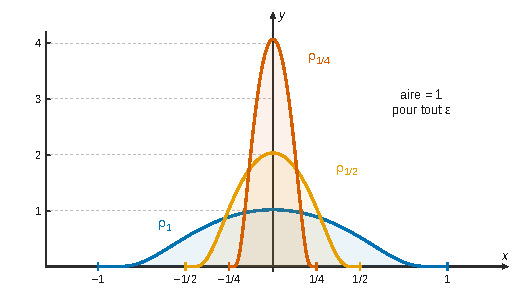
\includegraphics{figures/q6-bosses-rho-epsilon.pdf}
\caption*{Figure 1 --- Les bosses ρ\_ε pour ε = 1, 1/2, 1/4 : nulles pour
\textbar x\textbar{} \textgreater{} ε, de plus en plus hautes, toutes
d'aire 1}
\end{figure}

\hypertarget{q7}{%
\subsection{Q7}\label{q7}}

\textbf{(a)} La fonction \(\rho_\varepsilon g\) est continue et nulle hors de \([-\varepsilon,\varepsilon]\). Par Q6 et la positivité de \(\rho_\varepsilon\) :
\equationajustee{\begin{aligned}
\left|\int_{-\infty}^{+\infty}\rho_\varepsilon g-g(0)\right|&=\left|\int_{-\varepsilon}^{\varepsilon}\rho_\varepsilon(x)\big(g(x)-g(0)\big)\mathrm dx\right|\\
&\leqslant\omega(\varepsilon)\int_{-\varepsilon}^{\varepsilon}\rho_\varepsilon\\
&=\omega(\varepsilon),
\end{aligned}}
où \(\omega(\varepsilon)=\sup_{|x|\leqslant\varepsilon}|g(x)-g(0)|\) (fini : fonction continue sur un segment).

Soit \(\eta>0\). La fonction \(g\) est continue en \(0\). Il existe donc \(\alpha>0\) tel que \(|x|\leqslant\alpha\Rightarrow|g(x)-g(0)|\leqslant\eta\).

Donc \(\omega(\varepsilon)\leqslant\eta\) pour \(0<\varepsilon\leqslant\alpha\). Ainsi
\equationajustee{\boxed{\lim_{\varepsilon\to0^+}\int_{-\infty}^{+\infty}\rho_\varepsilon(x)g(x)\,\mathrm dx=g(0)}}

\textbf{(b)} Par le changement de variable \(t=x-a\) :
\equationajustee{\int\rho_\varepsilon(x-a)g(x)\,\mathrm dx=\int\rho_\varepsilon(t)\,g(a+t)\,\mathrm dt.}
La fonction \(h:t\mapsto g(a+t)\) est continue. Le (a) appliqué à \(h\) donne une limite \(h(0)=g(a)\) :
\equationajustee{\boxed{\lim_{\varepsilon\to0^+}\int_{-\infty}^{+\infty}\rho_\varepsilon(x-a)g(x)\,\mathrm dx=g(a)}}

\hypertarget{partie-b-distribution-sur-mathbb-r}{%
\section{\texorpdfstring{Partie B -- Distribution sur \(\mathbb R\)}{Partie B -- Distribution sur \textbackslash mathbb R}}\label{partie-b-distribution-sur-mathbb-r}}

\hypertarget{q8}{%
\subsection{Q8}\label{q8}}

\(\mathcal D'(\mathbb R)\) est une partie de l'espace vectoriel \(\mathcal F(\mathcal D(\mathbb R),\mathbb R)\) des applications de \(\mathcal D(\mathbb R)\) dans les réels. Elle contient l'application nulle (linéaire, avec \(C_K=1\) et \(N_K=0\)).

Soient \(T,S\in\mathcal D'(\mathbb R)\) et \(\lambda\in\mathbb R\). L'application \(T+\lambda S\) est linéaire.

Pour un segment \(K\), soient \((C_K,N_K)\) et \((C_K',N_K')\) les constantes respectives des deux distributions.

On pose \(N=\max(N_K,N_K')\) et \(C=C_K+|\lambda|C_K'>0\). Pour toute \(\varphi\in\mathcal D(K)\) :
\equationajustee{\begin{aligned}
|(T+\lambda S)(\varphi)|&\leqslant C_K\max_{i\leqslant N_K}\|\varphi^{(i)}\|_\infty+|\lambda|C_K'\max_{i\leqslant N_K'}\|\varphi^{(i)}\|_\infty\\
&\leqslant C\max_{i\leqslant N}\|\varphi^{(i)}\|_\infty.
\end{aligned}}
Donc \(T+\lambda S\in\mathcal D'(\mathbb R)\) : \textbf{\(\mathcal D'(\mathbb R)\) est un sous-espace vectoriel de \(\mathcal F(\mathcal D(\mathbb R),\mathbb R)\), donc un espace vectoriel.}

\hypertarget{q9}{%
\subsection{Q9}\label{q9}}

\(\delta_a\) est linéaire : \((f+\lambda g)(a)=f(a)+\lambda g(a)\).

Pour tout segment \(K\) et toute \(\varphi\in\mathcal D(K)\), on a \(|\delta_a(\varphi)|=|\varphi(a)|\leqslant\|\varphi\|_\infty\). Les constantes \(C_K=1\) et \(N_K=0\) conviennent : \textbf{\(\delta_a\in\mathcal D'(\mathbb R)\).}

\hypertarget{q10}{%
\subsection{Q10}\label{q10}}

Soit \(\varphi\in\mathcal D(\mathbb R)\) nulle hors de \([-A,A]\). Le produit \(f\varphi\) est continu par morceaux et nul hors de \([-A,A]\), donc intégrable sur \(\mathbb R\).

De plus \(T_f(\varphi)=\int_{-A}^Af\varphi\). Ainsi \(T_f\) est bien définie, et linéaire par linéarité de l'intégrale.

Pour un segment \(K\) et \(\varphi\in\mathcal D(K)\) :
\equationajustee{\begin{aligned}
|T_f(\varphi)|=\left|\int_Kf\varphi\right|&\leqslant\left(\int_K|f|\right)\|\varphi\|_\infty\\
&\leqslant C_K\|\varphi\|_\infty,
\end{aligned}}
avec \(C_K=1+\int_K|f|>0\) et \(N_K=0\). \textbf{\(T_f\in\mathcal D'(\mathbb R)\).}

\hypertarget{q11}{%
\subsection{Q11}\label{q11}}

Soit \(a\in\mathbb R\) et \(\varepsilon>0\). La fonction \(\theta_\varepsilon:x\mapsto\rho_\varepsilon(x-a)\) est \(\mathcal C^\infty\) et nulle pour \(|x|>|a|+\varepsilon\). Donc \(\theta_\varepsilon\in\mathcal D(\mathbb R)\).

L'égalité \(T_{f_1}(\theta_\varepsilon)=T_{f_2}(\theta_\varepsilon)\) s'écrit
\equationajustee{\int_{-\infty}^{+\infty}\rho_\varepsilon(x-a)f_1(x)\,\mathrm dx=\int_{-\infty}^{+\infty}\rho_\varepsilon(x-a)f_2(x)\,\mathrm dx.}
Les fonctions \(f_1\) et \(f_2\) sont continues. Quand \(\varepsilon\to0^+\), Q7 (b) donne l'égalité \(f_1(a)=f_2(a)\). Ceci pour tout \(a\) : \textbf{\(f_1=f_2\).}

\hypertarget{q12}{%
\subsection{Q12}\label{q12}}

\textbf{(a)} Soit \(x\neq0\). La fonction \(t\mapsto\varphi(tx)/x\) est une primitive de \(t\mapsto\varphi'(tx)\) sur \([0,1]\), donc
\equationajustee{\int_0^1\varphi'(tx)\,\mathrm dt=\dfrac{\varphi(x)-\varphi(0)}{x}=\psi(x).}
Si \(x=0\), \(\int_0^1\varphi'(0)\,\mathrm dt=\varphi'(0)=\psi(0)\).
\equationajustee{\boxed{\forall x\in\mathbb R,\ \psi(x)=\int_0^1\varphi'(tx)\,\mathrm dt}}

\textbf{(b)} Soit \(F(x,t)=\varphi'(tx)\) sur \(\mathbb R\times[0,1]\) et \(k\in\mathbb N^*\). Pour tout \(t\), \(x\mapsto F(x,t)\) est \(\mathcal C^k\) avec
\equationajustee{\dfrac{\partial^jF}{\partial x^j}(x,t)=t^j\varphi^{(j+1)}(tx).}
Ces fonctions sont continues en \(t\) sur le segment \([0,1]\), donc intégrables. De plus,
\equationajustee{\left|\frac{\partial^kF}{\partial x^k}(x,t)\right|\leqslant\|\varphi^{(k+1)}\|_\infty,}
constante intégrable sur \([0,1]\).

Par le théorème de dérivation des intégrales à paramètre (classe \(\mathcal C^k\)), \(\psi\) est \(\mathcal C^k\) sur la droite réelle, avec
\equationajustee{\psi^{(k)}(x)=\int_0^1t^k\varphi^{(k+1)}(tx)\,\mathrm dt.}
Ceci pour tout \(k\) : \textbf{\(\psi\in\mathcal C^\infty(\mathbb R)\).}

\hypertarget{q13}{%
\subsection{Q13}\label{q13}}

\textbf{(a)} Soit \(\varphi\in\mathcal D(\mathbb R)\) nulle hors de \([-A,A]\), et \(0<\varepsilon<A\). Les intégrales
\equationajustee{\int_{-\infty}^{-\varepsilon}\frac{\varphi(x)}x\mathrm dx=\int_{-A}^{-\varepsilon}\frac{\varphi(x)}x\mathrm dx}
et
\equationajustee{\int_\varepsilon^{+\infty}\frac{\varphi(x)}x\mathrm dx=\int_\varepsilon^A\frac{\varphi(x)}x\mathrm dx}
existent (fonctions continues sur des segments).

Pour \(x\neq0\), \(\dfrac{\varphi(x)}x=\dfrac{\varphi(0)}x+\psi(x)\), et
\equationajustee{\begin{aligned}
\int_{-A}^{-\varepsilon}\frac{\mathrm dx}x+\int_\varepsilon^A\frac{\mathrm dx}x&=\ln\frac\varepsilon A+\ln\frac A\varepsilon\\
&=0.
\end{aligned}}
Donc
\equationajustee{\begin{aligned}
J(\varepsilon)&=\int_{-A}^{-\varepsilon}\psi+\int_\varepsilon^A\psi\\
&=\int_{-A}^A\psi-\int_{-\varepsilon}^\varepsilon\psi.
\end{aligned}}
\(\psi\) est continue (Q12), donc bornée par \(M\) sur \([-A,A]\). Ainsi \(\left|\int_{-\varepsilon}^\varepsilon\psi\right|\leqslant2\varepsilon M\to0\). La limite existe :
\equationajustee{\boxed{\begin{aligned}V(\varphi)&=\int_{-A}^A\psi(x)\,\mathrm dx\\&=\int_{-A}^{A}\frac{\varphi(x)-\varphi(0)}{x}\,\mathrm dx\end{aligned}}}
(pour tout \(A\) tel que \(\varphi\) soit nulle hors de \([-A,A]\)).

\begin{figure}[H]
\centering
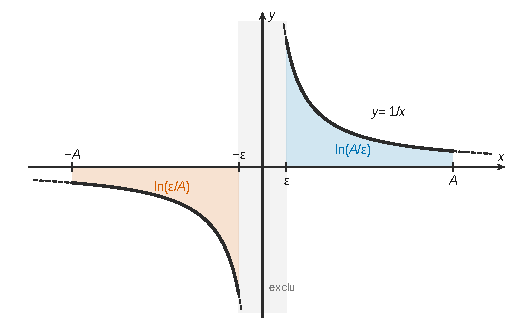
\includegraphics{figures/q13-valeur-principale.pdf}
\caption*{Figure 2 --- Valeur principale de 1/x : avec la découpe symétrique, les
aires ln(A/ε) et ln(ε/A) se compensent exactement}
\end{figure}

\textbf{(b)} \emph{Linéarité.} Pour \(\varepsilon>0\), l'application \(J_\varepsilon:\varphi\mapsto\int_{-\infty}^{-\varepsilon}\frac\varphi x+\int_\varepsilon^{+\infty}\frac\varphi x\) est linéaire. Les limites existant, \(V=\lim J_\varepsilon\) est linéaire.

\emph{Estimation.} Soit \(K=[\alpha,\beta]\) et \(a=\max(1,|\alpha|,|\beta|)\), de sorte que \(K\subset[-a,a]\). Pour \(\varphi\in\mathcal D(K)\), (a) donne \(V(\varphi)=\int_{-a}^a\psi\). Par Q12 (a),
\equationajustee{|\psi(x)|\leqslant\int_0^1|\varphi'(tx)|\,\mathrm dt\leqslant\|\varphi'\|_\infty.}
D'où
\equationajustee{\begin{aligned}
|V(\varphi)|&\leqslant2a\|\varphi'\|_\infty\\
&\leqslant2a\max_{i\in[\![0,1]\!]}\|\varphi^{(i)}\|_\infty.
\end{aligned}}
Les constantes \(C_K=2a>0\) et \(N_K=1\) conviennent : \textbf{\(V\in\mathcal D'(\mathbb R)\).}

\hypertarget{partie-c-duxe9rivation-dune-distribution}{%
\section{Partie C -- Dérivation d'une distribution}\label{partie-c-duxe9rivation-dune-distribution}}

\hypertarget{q14}{%
\subsection{Q14}\label{q14}}

Soit \(K\) un segment et \(\varphi\in\mathcal D(K)\). La fonction est nulle sur l'ouvert \(\mathbb R\setminus K\), donc sa dérivée aussi : \(\varphi'\in\mathcal D(K)\).

En particulier \(\varphi'\in\mathcal D(\mathbb R)\) pour toute \(\varphi\in\mathcal D(\mathbb R)\).

Donc \(T'\) est bien définie, et elle est linéaire comme composée de \(\varphi\mapsto\varphi'\) et de \(-T\). Avec les constantes \((C_K,N_K)\) de \(T\) :
\equationajustee{\begin{aligned}
|T'(\varphi)|=|T(\varphi')|&\leqslant C_K\max_{0\leqslant i\leqslant N_K}\|\varphi^{(i+1)}\|_\infty\\
&\leqslant C_K\max_{0\leqslant i\leqslant N_K+1}\|\varphi^{(i)}\|_\infty.
\end{aligned}}
Le couple \((C_K,N_K+1)\) convient : \textbf{\(T'\in\mathcal D'(\mathbb R)\).}

\hypertarget{q15}{%
\subsection{Q15}\label{q15}}

Soit \(\varphi\in\mathcal D(\mathbb R)\) nulle hors de \([-A,A]\). Les fonctions \(f\) et \(\varphi\) sont \(\mathcal C^1\) sur ce segment.

Par intégration par parties et \(\varphi(\pm A)=0\) :
\equationajustee{\begin{aligned}
T_f'(\varphi)&=-\int_{-A}^Af\varphi'\\
&=-\big[f\varphi\big]_{-A}^A+\int_{-A}^Af'\varphi\\
&=\int_{-\infty}^{+\infty}f'\varphi\\
&=T_{f'}(\varphi).
\end{aligned}}
\equationajustee{\boxed{T_f'=T_{f'}}}

\hypertarget{q16}{%
\subsection{Q16}\label{q16}}

\textbf{(a)} Le taux d'accroissement \(\dfrac{|x|-0}{x}\) vaut \(1\) pour \(x>0\).

Il vaut \(-1\) pour \(x<0\) : il n'a pas de limite en \(0\).

\textbf{\(f\) n'est pas dérivable en \(0\), donc pas sur \(\mathbb R\).}

\textbf{(b)} Soit \(\varphi\in\mathcal D(\mathbb R)\) nulle hors de \([-A,A]\). On intègre par parties sur \([-A,0]\) et \([0,A]\).

Les crochets sont nuls en \(0\) grâce au facteur \(x\). Ils sont nuls en \(\pm A\) car \(\varphi(\pm A)=0\) :
\equationajustee{\int_0^Ax\varphi'(x)\,\mathrm dx=-\int_0^A\varphi,}
\equationajustee{\int_{-A}^0(-x)\varphi'(x)\,\mathrm dx=\int_{-A}^0\varphi.}
Donc
\equationajustee{\begin{aligned}
T_f'(\varphi)&=-\int_{-A}^A|x|\varphi'(x)\,\mathrm dx\\
&=\int_0^A\varphi-\int_{-A}^0\varphi.
\end{aligned}}
On note \(\operatorname{sgn}\) la fonction signe :
\equationajustee{\operatorname{sgn}(x)=\begin{cases}1&x>0\\-1&x<0\\0&x=0\end{cases}}
Elle est continue par morceaux, et :
\equationajustee{\boxed{\begin{aligned}T_f'&=T_{\operatorname{sgn}}\\ T_f'(\varphi)&=\int_{-\infty}^{+\infty}\operatorname{sgn}(x)\varphi(x)\,\mathrm dx\end{aligned}}}
(la valeur en \(0\) est indifférente).

\hypertarget{q17}{%
\subsection{Q17}\label{q17}}

\(H\) est constante sur \(]-\infty,0[\) et sur \([0,+\infty[\). Elle a des limites finies à gauche et à droite en \(0\). Sur tout segment, elle a donc au plus une discontinuité, avec limites finies : elle est continue par morceaux.

Pour \(\varphi\in\mathcal D(\mathbb R)\) nulle hors de \([-A,A]\) :
\equationajustee{\begin{aligned}
T_H'(\varphi)&=-\int_0^A\varphi'(x)\,\mathrm dx\\
&=-\big(\varphi(A)-\varphi(0)\big)\\
&=\varphi(0)\\
&=\delta_0(\varphi).
\end{aligned}}
\equationajustee{\boxed{T_H'=\delta_0}}

\begin{figure}[H]
\centering
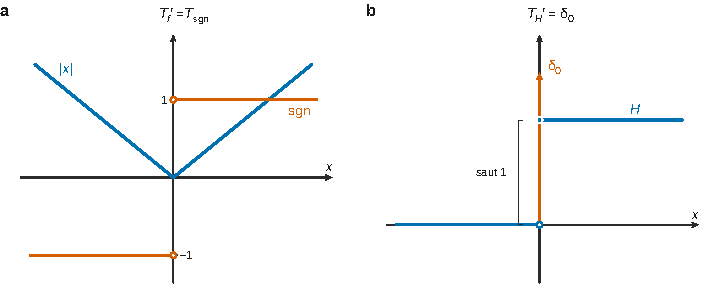
\includegraphics{figures/q17-saut-heaviside-dirac.pdf}
\caption*{Figure 3 --- Dérivées au sens des distributions : \textbar x\textbar{} a
pour dérivée la fonction signe (a), l'échelon H a pour dérivée la masse
de Dirac δ₀, égale au saut (b)}
\end{figure}

\hypertarget{q18}{%
\subsection{Q18}\label{q18}}

\textbf{(a)} \(T'=0\) signifie \(T'(\varphi)=-T(\varphi')=0\) pour toute \(\varphi\in\mathcal D(\mathbb R)\). D'où \textbf{\(T(\varphi')=0\).}

\textbf{(b)} Soit \(\varphi\) nulle hors de \([-A,A]\) et d'intégrale nulle. On pose \(\psi(x)=\int_{-\infty}^x\varphi(t)\,\mathrm dt\) (intégrale d'une fonction continue à support borné).

\(\psi\) est la primitive de \(\varphi\) nulle en \(-A\). Donc \(\psi'=\varphi\) et \(\psi\in\mathcal C^\infty(\mathbb R)\).

Pour \(x\leqslant-A\), \(\psi(x)=0\). Pour \(x\geqslant A\), \(\psi(x)=\int_{-\infty}^{+\infty}\varphi=0\).

Donc \(\psi\in\mathcal D(\mathbb R)\) et, par (a), \textbf{\(T(\varphi)=T(\psi')=0\).}

\textbf{(c)} \(\varphi_0=\rho_1\) convient : \(\rho_1\in\mathcal D(\mathbb R)\) (Q5) et \(\int\rho_1=1\) (Q6).

\textbf{(d)} Soit \(\alpha=\int\varphi\) et \(\chi=\varphi-\alpha\varphi_0\in\mathcal D(\mathbb R)\), d'intégrale \(\alpha-\alpha=0\). Par (b), \(T(\chi)=0\), et par linéarité :
\equationajustee{\boxed{\begin{aligned}T(\varphi)&=\alpha\,T(\varphi_0)\\&=T(\varphi_0)\int_{-\infty}^{+\infty}\varphi(t)\,\mathrm dt\end{aligned}}}

\textbf{(e)} Soit \(h\) la fonction constante égale à \(c=T(\varphi_0)\), continue. Pour toute \(\varphi\), \(T_h(\varphi)=c\int\varphi=T(\varphi)\) par (d). \textbf{\(T=T_h\) avec \(h\) constante.}

\hypertarget{q19}{%
\subsection{Q19}\label{q19}}

Soit \(f\) continue telle que \(T_f'=0\). Q18 (e) donne une constante \(h\) telle que \(T_f=T_h\).

Les fonctions \(f\) et \(h\) étant continues, Q11 donne \(f=h\).

Réciproquement, si \(f\) est constante, Q15 donne \(T_f'=T_{f'}=T_0=0\). \textbf{Les solutions sont les fonctions constantes.}

\hypertarget{q20}{%
\subsection{Q20}\label{q20}}

Soit \(f\) continue telle que \(T_f''=(T_f')'=0\). Comme \(T_f'\in\mathcal D'(\mathbb R)\) (Q14), Q18 (e) fournit \(c\in\mathbb R\) tel que \(T_f'=T_c\).

Soit \(g:x\mapsto cx\), de classe \(\mathcal C^1\) : \(T_g'=T_{g'}=T_c\) (Q15). Les applications \(u\mapsto T_u\) et \(T\mapsto T'\) étant linéaires,
\equationajustee{\begin{aligned}
(T_{f-g})'&=T_f'-T_g'\\
&=0.
\end{aligned}}
\(f-g\) est continue, donc constante égale à un réel \(d\) par Q19 : \(f(x)=cx+d\).

Réciproquement, si \(f\) est affine, deux applications de Q15 donnent \(T_f''=(T_{f'})'=T_{f''}=T_0=0\).

\equationajustee{\boxed{\{f\in\mathcal C^0(\mathbb R,\mathbb R):T_f''=0\}=\{x\mapsto cx+d,\ (c,d)\in\mathbb R^2\}}}

\hypertarget{q21}{%
\subsection{Q21}\label{q21}}

\(g\) est continue sur l'intervalle \(\mathbb R\). Par le théorème fondamental de l'analyse, \(G:x\mapsto\int_0^xg(t)\,\mathrm dt\) est de classe \(\mathcal C^1\) sur \(\mathbb R\). Et \textbf{\(G'=g\)}.

\hypertarget{q22}{%
\subsection{Q22}\label{q22}}

\(G\) étant \(\mathcal C^1\), Q15 donne \(T_G'=T_{G'}=T_g\). Par linéarité de la dérivation et l'hypothèse \(T_f'=T_g\) :
\equationajustee{\begin{aligned}
(T_f-T_G)'&=T_g-T_g\\
&=0.
\end{aligned}}
\equationajustee{\boxed{(T_f-T_G)'=0}}

\hypertarget{q23}{%
\subsection{Q23}\label{q23}}

\(T_f-T_G=T_{f-G}\), et \(f-G\) est continue. Par Q22 et Q19, \(f-G\) est une constante \(c\). Donc \(f=G+c\) :
\equationajustee{\boxed{f\in\mathcal C^1(\mathbb R)\ \text{et}\ f'=g}}

\hypertarget{partie-d-suite-de-distributions}{%
\section{Partie D -- Suite de distributions}\label{partie-d-suite-de-distributions}}

\hypertarget{q24}{%
\subsection{Q24}\label{q24}}

Soit \(\varphi\in\mathcal D(\mathbb R)\). On a \(\varphi'\in\mathcal D(\mathbb R)\) (Q14), donc \(T_n(\varphi')\to T(\varphi')\) et
\equationajustee{T_n'(\varphi)=-T_n(\varphi')\longrightarrow-T(\varphi')=T'(\varphi).}
\textbf{\(\lim T_n'\overset{\mathcal D}{=}T'\).}

\hypertarget{q25}{%
\subsection{Q25}\label{q25}}

On prend \(f_n(x)=\cos(nx)\), continue.

\begin{itemize}
\tightlist
\item
  En \(x=\pi\), \(f_n(\pi)=(-1)^n\) n'a pas de limite. Donc \((f_n)\) ne converge pas simplement sur \(\mathbb R\).
\item
  Soit \(\varphi\in\mathcal D(\mathbb R)\) nulle hors de \([-A,A]\) et \(n\geqslant1\). Par intégration par parties (\(\varphi(\pm A)=0\)) :
  \equationajustee{\begin{aligned}
  T_{f_n}(\varphi)&=\int_{-A}^A\cos(nx)\varphi(x)\,\mathrm dx\\
  &=\left[\frac{\sin(nx)}n\varphi(x)\right]_{-A}^A-\frac1n\int_{-A}^A\sin(nx)\varphi'(x)\,\mathrm dx,
  \end{aligned}}
  donc \(|T_{f_n}(\varphi)|\leqslant\dfrac{2A\|\varphi'\|_\infty}{n}\to0\).
\end{itemize}

\textbf{La suite \((x\mapsto\cos(nx))_n\) convient} : elle ne converge pas simplement et \(\lim T_{f_n}\overset{\mathcal D}{=}0\).

\hypertarget{q26}{%
\subsection{Q26}\label{q26}}

Soit \(\varphi\in\mathcal D(\mathbb R)\) nulle hors de \([-A,A]\). Soit \(n\) assez grand pour que \(f_n-f\) soit bornée :
\equationajustee{\begin{aligned}
|T_{f_n}(\varphi)-T_f(\varphi)|&\leqslant\int_{-A}^A|f_n-f|\,|\varphi|\\
&\leqslant2A\|\varphi\|_\infty\|f_n-f\|_\infty\xrightarrow[n\to+\infty]{}0.
\end{aligned}}
\textbf{\(\lim T_{f_n}\overset{\mathcal D}{=}T_f\).}

\hypertarget{q27}{%
\subsection{Q27}\label{q27}}

Soit \(\varphi\in\mathcal D(\mathbb R)\) nulle hors de \([-A,A]\). On applique l'inégalité de Cauchy-Schwarz sur le segment \([-A,A]\), puis la positivité de \((f_n-f)^2\) :
\equationajustee{\begin{aligned}
|T_{f_n}(\varphi)-T_f(\varphi)|&\leqslant\left(\int_{-A}^A(f_n-f)^2\right)^{1/2}\left(\int_{-A}^A\varphi^2\right)^{1/2}\\
&\leqslant\|f_n-f\|_2\left(\int_{-A}^A\varphi^2\right)^{1/2}\xrightarrow[n\to+\infty]{}0.
\end{aligned}}
\textbf{\(\lim T_{f_n}\overset{\mathcal D}{=}T_f\).}

\hypertarget{partie-e-une-application-le-thuxe9oruxe8me-dunicituxe9-de-cantor}{%
\section{Partie E -- Une application, le théorème d'unicité de Cantor}\label{partie-e-une-application-le-thuxe9oruxe8me-dunicituxe9-de-cantor}}

On note \(u_n(x)=a_n\cos(nx)+b_n\sin(nx)\) et \(S_N=\sum_{n=1}^Nu_n\). Par hypothèse, \(S_N(x)\to0\) pour tout \(x\in\mathbb R\).

\begin{figure}[H]
\centering
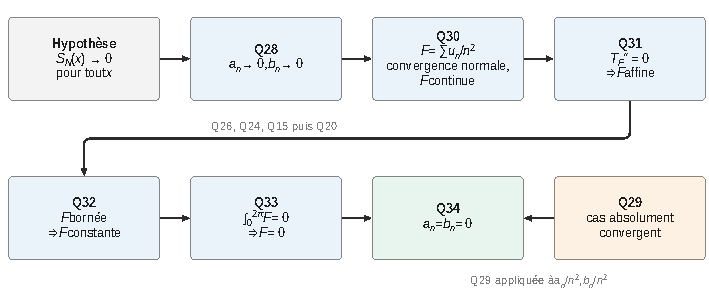
\includegraphics{figures/partie-e-strategie.pdf}
\caption*{Figure 4 --- Enchaînement de la partie E : de l'hypothèse S\_N → 0 aux
coefficients nuls, via F = ∑ u\_n/n² et le cas absolument convergent
(Q29)}
\end{figure}

\hypertarget{q28}{%
\subsection{Q28}\label{q28}}

\textbf{(a)} En \(x=0\), \(u_n(0)=a_n\). La série \(\sum a_n\) converge, donc son terme général tend vers \(0\) : \textbf{\(a_n\to0\).}

\textbf{(b)} Pour tout \(x\), \(u_n(x)\to0\) (terme général d'une série convergente) et \(|a_n\cos(nx)|\leqslant|a_n|\to0\). Par différence, \textbf{\(b_n\sin(nx)\to0\) pour tout \(x\in\mathbb R\)}, en particulier sur \([0,2\pi]\).

\textbf{(c)} Supposons que \((b_n)\) ne tend pas vers \(0\). Il existe alors \(\varepsilon>0\) tel que \(|b_n|\geqslant\varepsilon\) pour une infinité d'indices.

Il y a alors une infinité d'indices avec \(b_n\geqslant\varepsilon\), ou une infinité avec \(b_n\leqslant-\varepsilon\).

Dans le second cas, on remplace \((a_n,b_n)\) par \((-a_n,-b_n)\). Cela conserve l'hypothèse (série convergente de somme nulle en tout point) et ne change pas la convergence de \((b_n)\) vers \(0\).

L'ensemble \(E=\{n\in\mathbb N^*:b_n\geqslant\varepsilon\}\) est donc infini. On définit par récurrence
\equationajustee{\begin{aligned}\varphi(0)&=\min E\\ \varphi(n+1)&=\min\{m\in E:m>\varphi(n)\}\end{aligned}}
ce minimum existant car \(E\) est infini. Alors \textbf{\(\varphi:\mathbb N\to\mathbb N^*\) est strictement croissante et \(b_{\varphi(n)}\geqslant\varepsilon\) pour tout \(n\).}

\textbf{(d)} Soit \(x\in[0,2\pi]\). La suite \(\big(b_{\varphi(n)}\sin(\varphi(n)x)\big)_n\) est extraite de \(\big(b_m\sin(mx)\big)_m\), qui tend vers \(0\) par (b). Comme \(b_{\varphi(n)}^2\geqslant\varepsilon^2\),
\equationajustee{\begin{aligned}
0\leqslant\sin^2(\varphi(n)x)&\leqslant\frac{\big(b_{\varphi(n)}\sin(\varphi(n)x)\big)^2}{\varepsilon^2}\\
&\longrightarrow0.
\end{aligned}}
Les fonctions continues \(g_n:x\mapsto\sin^2(\varphi(n)x)\) convergent donc simplement vers \(0\) sur \([0,2\pi]\). Elles vérifient \(|g_n|\leqslant1\), fonction intégrable sur le segment. Par le théorème de convergence dominée :
\equationajustee{\boxed{\lim_{n\to+\infty}\int_0^{2\pi}\sin^2(\varphi(n)x)\,\mathrm dx=0}}

\textbf{(e)} Pour \(k\in\mathbb N^*\),
\equationajustee{\begin{aligned}
\int_0^{2\pi}\sin^2(kx)\,\mathrm dx&=\int_0^{2\pi}\frac{1-\cos(2kx)}2\,\mathrm dx\\
&=\pi.
\end{aligned}}
La suite du (d) est donc constante égale à \(\pi\neq0\) : contradiction. \textbf{Donc \(b_n\to0\)}, et avec (a), \(a_n\to0\) et \(b_n\to0\).

\hypertarget{q29}{%
\subsection{Q29}\label{q29}}

Pour tout \(x\), \(|u_n(x)|\leqslant|a_n|+|b_n|\), terme général d'une série convergente. Donc \(\sum u_n\) converge normalement, donc uniformément, sur \(\mathbb R\), et sa somme est nulle.

Soit \(k\in\mathbb N^*\). La série \(\sum u_n\cos(k\,\cdot)\) converge uniformément sur \([0,2\pi]\), car \(|\cos|\leqslant1\). Ses termes sont continus. On peut donc l'intégrer terme à terme sur ce segment. Par linéarisation, pour \(n,k\in\mathbb N^*\) (avec \(n+k\neq0\)) :
\equationajustee{\int_0^{2\pi}\cos(nx)\cos(kx)\,\mathrm dx=\pi\,\delta_{n,k},}
\equationajustee{\int_0^{2\pi}\sin(nx)\cos(kx)\,\mathrm dx=0,}
\equationajustee{\int_0^{2\pi}\sin(nx)\sin(kx)\,\mathrm dx=\pi\,\delta_{n,k}.}
Donc
\equationajustee{\begin{aligned}
0&=\int_0^{2\pi}\Big(\sum_{n=1}^{+\infty}u_n(x)\Big)\cos(kx)\,\mathrm dx\\
&=\sum_{n=1}^{+\infty}\int_0^{2\pi}u_n(x)\cos(kx)\,\mathrm dx\\
&=\pi a_k,
\end{aligned}}
et de même avec \(\sin(kx)\) : \(0=\pi b_k\).
\equationajustee{\boxed{\forall n\in\mathbb N^*,\ a_n=0\ \text{et}\ b_n=0}}

\hypertarget{q30}{%
\subsection{Q30}\label{q30}}

Par Q28, \((a_n)\) et \((b_n)\) convergent, donc sont bornées. Il existe ainsi \(M>0\) tel que \(|a_n|+|b_n|\leqslant M\) pour tout \(n\). Alors, pour tout \(x\in\mathbb R\),
\equationajustee{\begin{aligned}
|f_n(x)|&\leqslant\frac{|a_n|+|b_n|}{n^2}\\
&\leqslant\frac M{n^2},
\end{aligned}}
terme général d'une série de Riemann convergente : \textbf{\(\sum f_n\) converge normalement sur \(\mathbb R\).} En particulier la convergence est uniforme et \(F\) est continue sur \(\mathbb R\).

\hypertarget{q31}{%
\subsection{Q31}\label{q31}}

Soit \(F_N=\sum_{n=1}^Nf_n\), de classe \(\mathcal C^\infty\), avec \(F_N''=-\sum_{n=1}^N u_n=-S_N\). Deux applications de Q15 (à \(F_N\) puis à \(F_N'\)) donnent \(T_{F_N}''=T_{F_N''}=-T_{S_N}\).

\((F_N)\) converge uniformément vers \(F\) sur \(\mathbb R\) (Q30). Donc \(\lim T_{F_N}\overset{\mathcal D}{=}T_F\) (Q26).

Puis \(\lim T_{F_N}''\overset{\mathcal D}{=}T_F''\) (Q24 appliquée deux fois). Pour toute \(\varphi\in\mathcal D(\mathbb R)\) nulle hors de \([-A,A]\) :
\equationajustee{T_F''(\varphi)=-\lim_{N\to+\infty}\int_{-A}^AS_N(x)\varphi(x)\,\mathrm dx.}
Par hypothèse, \(S_N\varphi\to0\) simplement sur \([-A,A]\). En passant à la limite sous l'intégrale, on obtient \(T_F''(\varphi)=0\), donc \(T_F''=0\). \(F\) étant continue (Q30), Q20 donne :
\equationajustee{\boxed{F\text{ est affine : }F(x)=cx+d}}

\emph{Réserve.} Le passage à la limite sous l'intégrale est le point que le sujet admet implicitement : la convergence simple de \((S_N)\) ne suffit pas. Le théorème de convergence dominée exige une majoration \(|S_N|\leqslant g\) sur \([-A,A]\). Il faut \(g\) intégrable et indépendante de \(N\), ce que l'énoncé ne fournit pas. Cette majoration existe sous l'hypothèse de Q29 (\(|S_N|\leqslant\sum(|a_n|+|b_n|)\)). Dans le cas général, une preuve complète passe par les lemmes de Riemann et de Schwarz sur les dérivées secondes symétriques, hors programme.

\hypertarget{q32}{%
\subsection{Q32}\label{q32}}

Pour tout \(x\), \(|F(x)|\leqslant\sum_{n\geqslant1}M/n^2=M\pi^2/6\) : \textbf{\(F\) est bornée.}

Supposons \(F(x)=cx+d\) avec \(c\neq0\). Alors \(|F(x)|\to+\infty\) quand \(x\to+\infty\), ce qui est absurde.

Donc \(c=0\) : \textbf{\(F\) est constante, égale à \(d\).}

\hypertarget{q33}{%
\subsection{Q33}\label{q33}}

\(\sum f_n\) converge uniformément sur le segment \([0,2\pi]\) et ses termes sont continus : on peut intégrer terme à terme. Pour \(n\geqslant1\), on a \(\int_0^{2\pi}\cos(nx)\,\mathrm dx=0\) et \(\int_0^{2\pi}\sin(nx)\,\mathrm dx=0\), donc
\equationajustee{\begin{aligned}
2\pi d&=\int_0^{2\pi}F(x)\,\mathrm dx\\
&=\sum_{n=1}^{+\infty}\int_0^{2\pi}f_n(x)\,\mathrm dx\\
&=0.
\end{aligned}}
Donc \(d=0\) : \textbf{\(F=0\).}

\hypertarget{q34}{%
\subsection{Q34}\label{q34}}

Posons \(\alpha_n=a_n/n^2\) et \(\beta_n=b_n/n^2\). La série \(\sum(\alpha_n\cos(nx)+\beta_n\sin(nx))=\sum f_n(x)\) converge pour tout \(x\), de somme \(F(x)=0\) (Q30, Q33).

De plus, \(|\alpha_n|\leqslant M/n^2\) et \(|\beta_n|\leqslant M/n^2\). Donc \(\sum|\alpha_n|\) et \(\sum|\beta_n|\) convergent.

Q29 s'applique à \((\alpha_n)\) et \((\beta_n)\) : \(\alpha_n=\beta_n=0\), donc
\equationajustee{\boxed{\forall n\in\mathbb N^*,\ a_n=0\ \text{et}\ b_n=0}}

\textbf{Conclusion (théorème d'unicité de Cantor).} Une série trigonométrique \(\sum_{n\geqslant1}(a_n\cos(nx)+b_n\sin(nx))\) qui converge vers \(0\) en tout point de \(\mathbb R\) a tous ses coefficients nuls. Par différence, deux séries trigonométriques convergeant en tout point vers la même somme ont les mêmes coefficients : un développement trigonométrique partout convergent est unique.

\end{document}
